\chapter{Machine Learning Algorithms}
\noindent In most cases, machine learning algorithms are focused on building a model. Then, the model can be used to take inputs and give outputs based on the model. The model is a tool to predict outputs based on the inputs. In our case, we will be using models to take information about stocks and predict their future prices.
\begin{figure}[h]
\centering
\begin{tikzpicture}
  [node distance=.8cm,
  start chain=going below,]
  	\node (data) [punktchain] {Data};
    \node (ml) [punktchain, join=by {->}] {Machine Learning};
      \node (model) [punktchain, join=by {->}]  {Model};
      \begin{scope}[start branch=venstre,
        %We need to redefine the join-style to have the -> turn out right
        every join/.style={->, thick, shorten <=1pt}, ]
        \node[punktchain, on chain=going left, join=by {<-}]
            (inputs) {Observation $\vec{x}$};
      \end{scope}
      \begin{scope}[start branch=hoejre,]
      \node (finans) [punktchain, on chain=going right, join=by {->}] {Prediction y};
    \end{scope}
  % Now that we have finished the main figure let us add some "after-drawings"
  %% First, let us connect (finans) with (disk). We want it to have
  %% square corners.
\end{tikzpicture}
\end{figure}

\noindent So we use machine learning to take historical data and generate a model. When we want to use it, we give the model observations, $\vec{x_i}$, and it gives us predictions, $y$. Examples of good inputs (predictive factors) are:
\begin{enumerate}
	\item Price momentum
    \item Bollinger value
    \item Current price
\end{enumerate}
\noindent while examples of outputs would be:
\begin{enumerate}
	\item Future price
    \item Future return
\end{enumerate}
\noindent We'll first talk about Supervised Regression Learning.

\section{Regression and Modeling}
\noindent Supervised Regression Learning means that we'll provide (supervised learning) a bunch of example data $(x,y)_i$ and allow the model to make a numerical prediction (regression). There are two main types of regression techniques:
\begin{itemize}
\item Linear regression (parametric)
\item \ac{kNN} (instance-based), the more popular approach
\item Decision trees
\item Decision forests
\end{itemize}

\section{Assessing a Model}
Assessing a model is much like predicting prices as it uses indicators to judge the effectiveness of the model. The first indicator is \ac{rmse}, which is as follows
\begin{align*}
\sqrt{\frac{\sum(y_{test}-y_{predict})^2}{N}}
\end{align*}
The error that is important is that of test data, which is outside of the training data. Typically 60\% of the data is used for training, and 40\% is used for testing. However, sometimes there isn't enough data to adequately evaluate a learning algorithm, in which case a method called \textbf{cross validation} is used. This method slices the data into chunks, typically fifths. One is chosen as test and the rest are for training, then a different chunk is chosen to be the test and another trial is run. For financial data, we don't want to accidentally look forward in time, so we would only use \textbf{roll forward cross validation}. This simply demands that all the training data is before the test data. \\

The second metric for how well an algorithm is working is the \textbf{correlation} of the test data and predicted values. Strong correlation, close to $\pm$1, indicates a good algorithm whereas a weak correlation, close to zero, indicates a poor algorithm. Correlation and \ac{rmse} are excellent indicators on how well an algorithm is doing, but we might also want to fine tune an algorithm; we want to answer the question "when are we trying too hard to fit data?". This is where \textbf{overfitting} comes into play. Overfitting is the point at which error for training data is decreasing while error for test data is increasing.
\begin{figure}[h]
\centering
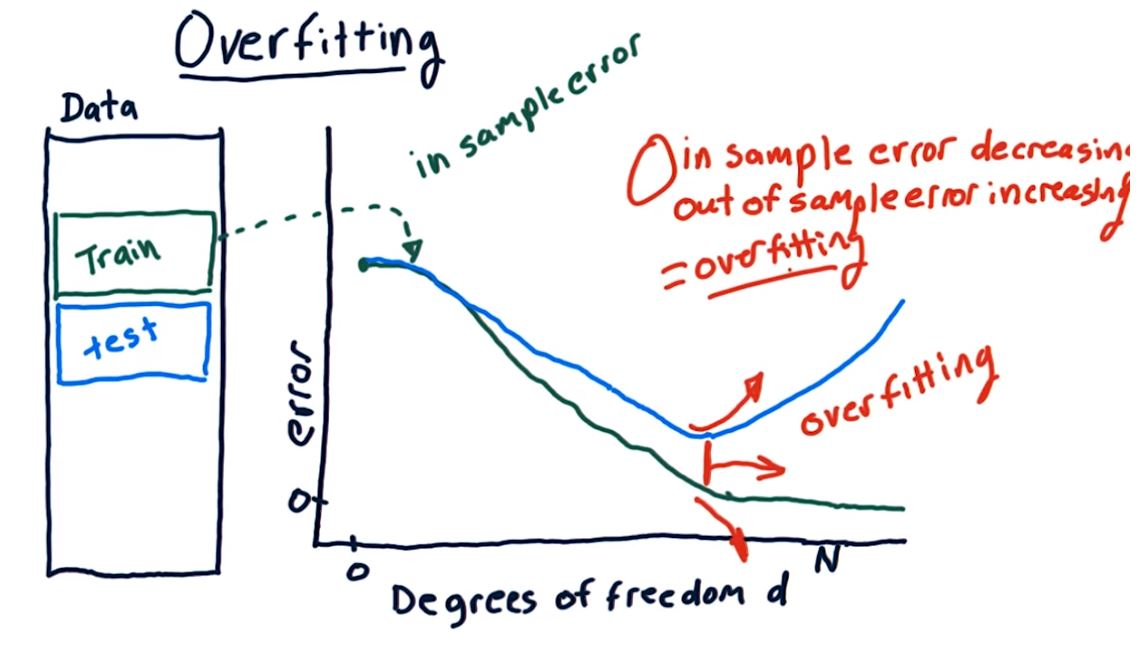
\includegraphics[scale=.6]{images/overfit.JPG}
\end{figure}

\section{Types of Learners}

\paragraph{Ensemble Learners}
Ensemble learners are composed of several different learners, which could include \ac{kNN}, regression, and decision tree learners in one. The output of this learner is then simply a combination of the learners' answers, which is typically an average of the outputs.

\paragraph{Bagging and Boosting}
Boot-strap aggregating, or \textbf{bagging}, only uses one algorithm, but many different models. If the training data is separated into learning instances where there's a total of $n$ instances, then each model is fed a bag of these instances. Each bag is composed of $n'$ learning instances that are randomly selected with replacement, so instances may show up more than once in the same bag. These are used to train $m$ models and the result is the average of all the outputs. \textbf{Boosting} builds each subsequent bag based on the results of the last. Training data is also used to test the models, and a model's predicted data showing significant error is weighted to more likely be in the next bag for the next model. The process is continued for the desired number of models, and the results are averaged. Although this could be advantageous in predicting outliers, it's also more susceptible to overfitting.

\subsection{Reinforcement Learning}
As seen in figure 4.1, reinforcement learning describes the interaction of a robot with its environment. The robot performs an action, which has an effect on the environment and changes its state. The robot observes the change in state and its associated reward and makes decisions to maximize that reward.

\begin{figure}[h]
\centering
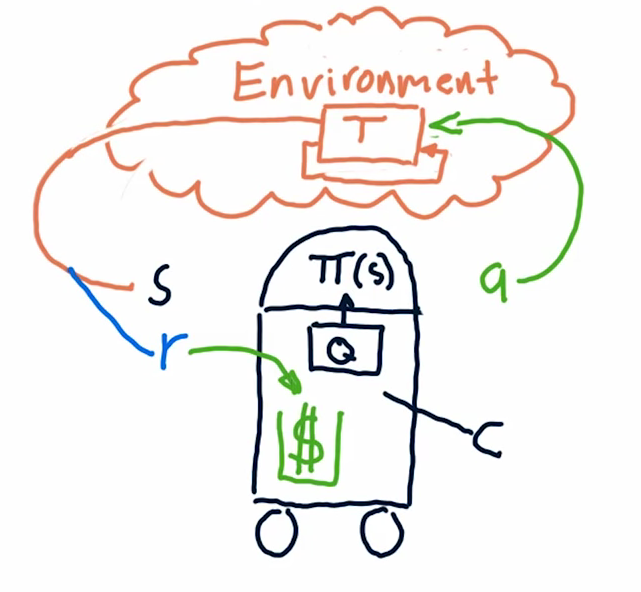
\includegraphics[width=6cm]{images/rl.png}
\caption{A diagram of how policy learning works}
\end{figure}

Reinforcement learning also describes the problem that is how to go about maximizing the reward. In the stock market, the reward is return on trades, and we want to find out how to maximize returns. This problem is complicated by time constraints. The value of future gains diminishes with time, so it's unreasonable to use an infinite horizon on which to base returns. However, optimizing returns over too short a time may limit rewards from seeing a much larger overall gain.

\subsection{Markov Decision Problems}
\noindent What we've been talking about is called a Markov decision problem. Here's how the problem is formalized.

We have:
\begin{itemize}
\item Set of states $S = \{s_1, \ldots, s_n\}$
\item Set of actions $A = \{a_1, \ldots, a_n\}$
\item Transition function $T[s,a,s']$
\item Reward function $R[s,a]$
\end{itemize}

\noindent What we're trying to find is a policy $\pi(s)$ that will maximize the reward. Unfortunately, we don't know the $T$ or $R$, since that's defined by the environment. So, the learner has to interact with the world and see what happens. Based on the reward, it can start generating policies.\\

\noindent A way to encode this information is using \textbf{experience tuples}. Experience tuples are as follows: given a state $s_1$ and an action $a_1$ that we took, we were put into state $s_1'$ and got reward $r_1$. The tuple is shown like this:

\begin{equation*}
\langle s_1, a_1, {s_1}', r_1 \rangle
\end{equation*}

\noindent Now, we can rename ${s_1}'$ to $s_2$, since that's our new state, and then take a new action and see what happens, and we get a new tuple:
\begin{equation*}
\langle s_2, a_2, {s_2}', r_2 \rangle
\end{equation*}

\noindent And we repeat this for many different combinations of states and actions, and then we'll use the tuples to generate the policy. There are two ways to generate the policy:

\paragraph{Model-based} For this method, we generate a model of $T[s,a,s']$ based on statistical analysis of the tuples. We look at a particular state and a particular action and see the probability of transitioning to another state. Same thing with $R[s,a]$. Then, we can use policy or value iteration to solve it.

\paragraph{Model-free} This method keeps the data around and uses the original tuples to determine what the new state will be for a certain action. This is Q-learning.

\section{Q-Learning}

\noindent Q-Learning is a model-free approach, which means that it doesn't need to have any sort of model of the transition function $T$ or the reward function $R$. It builds a table of \textit{utility values} as the agent interacts with the world. These are the Q values. At each state, the agent can then use the Q values to select the best action. Q-Learning is guaranteed to give an optimal policy, as it is proven to always converge.\\

\noindent Q represents the \textit{value} of taking action $a$ in state $s$. This value includes the immediate reward for taking action $a$, and the discounted (future) reward for all optimal future actions after having taken $a$. \\

\subsection{How do we use Q?}
\noindent What we want to find for a particular state is what policy, $\Pi(s)$ we should take. Using Q values, all we need to do is find the maximum Q value for that state.

\begin{equation}
\Pi(s) = {argmax}_{a}(Q[s,a])
\end{equation}

\noindent So, we go through each action $a$ and see which action has the maximum Q value for state $s$. Eventually, after learning enough, the agent will converge to the optimal policy, $\pi^*(s)$, and optimal Q table, $Q^*[s,a]$.

\subsection{How do we get Q?}
\noindent To use the Q table, first we must generate it by learning. How do we go about that? Well it's similar to previous learning algorithms, in that we provide it training data for which we know the outcomes. We then iterate over time and take actions based on the current policy ($Q$ values), and generate experience tuples $\langle s,a,s',r\rangle$ and generate the $Q$ values based on the experience.\par

\noindent In a more detailed fashion:

\begin{enumerate}
\item Initialize the $Q$ table with small random values
\item Compute $s$
\item Select $a$
\item Observe $r, s$
\item Update $Q$
\item Step forward in time, then repeat from step 2.
\end{enumerate}

\noindent To update $Q$, we first need a formula to decide what it should be. What we can do is assign a \textit{learning rate}, $\alpha$, to weight the new observations. We can therefore update $Q$ like this:

\begin{equation*}
Q'[s,a] = Q[s,a] + \alpha({improved\ estimate} - Q[s,a])
\end{equation*}

\noindent As you can see, $Q$ converges as the improved estimate is the same as the current estimate (we're at the best $Q$). Now, we need to know what the improved estimate is:

\begin{equation*}
improved\ estimate = immediate\ returns + (discounted\ future\ rewards)
\end{equation*}

\noindent Then, replacing \textit{discounted future rewards} with the actual way of calculating it, and rearranging to only use the current value of $Q$ once, we find that the formula to calculate the new value of Q for a state-action pair $\langle s,a\rangle$, the formula is:

\begin{equation}
Q'[s,a] = (1-\alpha)Q[s,a] + \alpha (r+\gamma\ Q[s',{argmax}_{a'}(Q[s',a'])])
\end{equation}

\noindent where:
\begin{itemize}
\item $r = R[s,a]$ is the \textit{immediate reward} for taking an action $a$ in the state $s$
\item $\gamma \in [0,1]$ is the \textit{discount factor} to reduce the value of future rewards
\item $s'$ is the resulting next state
\item ${argmax}_{a'}(Q[s',a'])$ is the action which maximizes the Q-value among all possible actions $a'$ from $s'$, and
\item $\alpha \in [0,1]$ is the \textit{learning rate} used to vary the weight given to new experiences compared to past Q-values. It's typically around 0.2.
\end{itemize}

\subsection{Exploration}
\noindent The success of a Q-learning algorithm depends on the exploration of the state-action space. If you only explore a small subset of it, you might not find the best policies. One way to ensure that you explore as much as possible is to introduce randomness into selecting actions during the learning phase. So basically, you see first whether you want to take the action with the maximal Q value or choose a random action, then if you take a random action, each action gets a probability which decreases over subsequent iterations.

\subsection{Q-Learning for Trading}
\noindent Now that we know what Q-learning is, we need to figure out how to apply it to the context of trading. That means that we need to define what \textit{state}, \textit{action}, and \textit{reward} mean. Actions are straightforward, as there are basically three of them:

\begin{itemize}
\item {\color{DarkerGreen} BUY}
\item {\color{red} SELL}
\item NOTHING
\end{itemize}

\noindent Our rewards can be daily returns or cumulative returns after a trade cycle (buy$\rightarrow$sell). However, using daily returns will allow the agent to converge on a $Q$ value more quickly, because if it waited until a sell, then it would have to look at all of the actions backwards until the buy to get that reward.\\

\noindent Now, we just need to figure out how to determine state. Some good factors to determine state are:

\begin{itemize}
\item Adjusted Close/Simple Moving Average
\item Bollinger Band value
\item P/E ratio
\item Holding stock (whether or not we're holding the stock)
\item Return since entry
\end{itemize}

\noindent Our state must be a single number so we can look it up in the table easily. To make it simpler, we'll confine the state to be an integer, which means we need to discretize each factor and then combine them into an overall state. Our state space is discrete, so the combined value is the overall state. Say we have a state like this:

\begin{table}[h]
\centering
\begin{tabular}{ccc}
\textbf{Factor} & \textbf{Value} & \textbf{Discretized}\\
$X_1$ & 25.6 & 0\\
$X_2$ & 0.3 & 5\\
$X_3$ & 2.0 & 9\\
$X_4$ & -5.1 & 2
\end{tabular}
\end{table}

\noindent The discretized state could be: 2950.

\paragraph{Discretization} To discretize, what we do is take the data for a factor over its range, then divide it into $n$ bins. Then we find the threshold by iterating over the data by the step size and taking the value at each position.

\begin{lstlisting}[style=python]
stepsize = size(data)/n
data.sort()
for i in range(0, steps):
	threshold[i] = data[(i+1)*stepsize]
\end{lstlisting}

\begin{figure}[h]
\centering
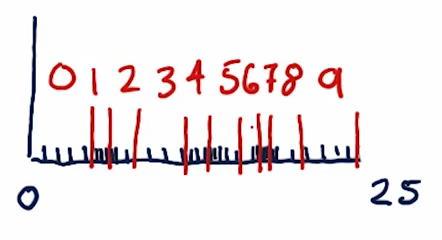
\includegraphics[width=6cm]{images/discretization.png}
\caption{What the thresholds might look like for a discretized data set if $n = 10$}
\end{figure}

\subsection{Problems with Q-Learning}
\noindent One main problem with Q-Learning is that it takes a lot of experience tuples to converge to the optimal Q value. This means the agent has to take many \textit{real} interactions with the world (execute trades) to learn. The way this has been addressed is by using \textit{Dyna}.

\section{Dyna-Q}

\noindent Dyna is designed to improve the convergence of Q learning by building a model of $T$ and $R$ and then using Q learning to make decisions based on the model. However, the Q learning portion is still model-free, so it's a mix of both.\\

\noindent So we do the Q-Learning steps, but after we take an action, we update the model of $T$ and $R$ with the new data, simulate a bunch of experiences based on the model, then update $Q$ based on these simulated experiences. To simulate the experiences, we basically generate random states and actions, and then find the new states/rewards based on the transition function and reward function.

\subsection{Learning $T$}

\noindent To figure out a model for T, what we can do is count the number of times that a transition to $s'$ by using the action $a$ in state $s$ occurred, then divide that by the total number of transitions to figure out the probability.

\begin{equation}
T[s,a,s'] = \frac{T_c[s,a,s']}{\sum_{i} T_c[s,a,i]}
\end{equation}

\noindent where $T_c$ is the number of times the transition occurred.

\subsection{Learning $R$}

\noindent To finalize the model, we need to find our expected reward, $R[s,a]$. Whenever we interact with the world, we get an immediate reward, $r$. We can use this to update our model for $R$ in a similar way to updating the Q values.

\begin{equation}
R'[s,a] = (1-\alpha)R[s,a] + \alpha r
\end{equation}

\noindent where $\alpha$ is, again, the learning rate.

\subsection{Conclusion}
\noindent So a summary of how Dyna-Q works is the following:

\begin{align*}
\noindent Q\ learning&\left\{
	\begin{tabular}{@{}l@{}}
    	init Q table\\
        observe S\\
        execute a, observe s;r\\
        update Q with $\langle s, a, s', r \rangle$\\
    \end{tabular}
\right.\\
\noindent Update\ model&\left\{
	\begin{tabular}{@{}l@{}}
    	update T'[s,a,s']\\
        update R'[s,a]
    \end{tabular}
\right.\\
\noindent Dyna\ Q&\left\{
	\begin{tabular}{@{}l@{}}
    	s = random\\
        a = random\\
        s' = infer from $T$\\
        r = R[s,a]\\
        update Q with new experience tuple\\
        repeat many times ($\sim100-200$)
    \end{tabular}
\right.
\end{align*}

\begin{figure}[h]
	\centering
	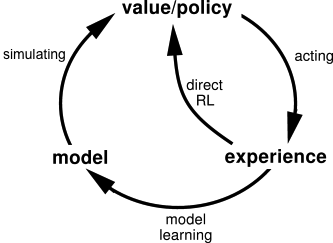
\includegraphics[width=7cm]{images/Dyna-architecture.png}
	\caption{A diagram of the Dyna architecture (courtesy Sutton and Barto)}
\end{figure}